\iffalse
\let\negmedspace\undefined
\let\negthickspace\undefined
\documentclass[journal,12pt,twocolumn]{IEEEtran}
\usepackage{cite}
\usepackage{amsmath,amssymb,amsfonts,amsthm}
\usepackage{algorithmic}
\usepackage{graphicx}
\usepackage{textcomp}
\usepackage{xcolor}
\usepackage{txfonts}
\usepackage{listings}
\usepackage{enumitem}
\usepackage{mathtools}
\usepackage{gensymb}
\usepackage{comment}
\usepackage[breaklinks=true]{hyperref}
\usepackage{tkz-euclide}
\usepackage{listings}
\usepackage{gvv}
\def\inputGnumericTable{}
\usepackage[latin1]{inputenc}
\usepackage{color}
\usepackage{array}
\usepackage{longtable}
\usepackage{calc}
\usepackage{multirow}
\usepackage{hhline}
\usepackage{ifthen}
\usepackage{lscape}

\newtheorem{theorem}{Theorem}[section]
\newtheorem{problem}{Problem}
\newtheorem{proposition}{Proposition}[section]
\newtheorem{lemma}{Lemma}[section]
\newtheorem{corollary}[theorem]{Corollary}
\newtheorem{example}{Example}[section]
\newtheorem{definition}[problem]{Definition}
\newcommand{\BEQA}{\begin{eqnarray}}
\newcommand{\EEQA}{\end{eqnarray}}
\newcommand{\define}{\stackrel{\triangle}{=}}
\theoremstyle{remark}
\newtheorem{rem}{Remark}
\begin{document}

\bibliographystyle{IEEEtran}
\vspace{3cm}

\title{NCERT Discrete - 11.9.3.12}
\author{EE23BTECH11058 - Sindam Ananya$^{*}$% <-this % stops a space
}
\maketitle
\newpage
\bigskip

\renewcommand{\thefigure}{\theenumi}
\renewcommand{\thetable}{\theenumi}

\vspace{3cm}
\textbf{Question : 11.9.3.12} 
The sum of the first three terms of a G.P is $39/10$ and their product is $1$. Find the common ratio and the terms.\\
\solution
\fi
\begin{table}[h!]
    \centering
    \begin{tabular}{|c|c|c|}
        \hline
        \textbf{Parameter} & \textbf{Value} & \textbf{Description} \\
        \hline
        $x(0)$ & & First term \\
        \hline
        $r$ & & Common ratio \\
        \hline
        $x(0)^3r^3$ & 1 & Product of terms \\
        \hline
        $x(0)$ + $x(0)r$ + $x(0)r^2$ & $\frac{39}{10}$ & Sum of terms \\
        \hline
    \end{tabular}

    \caption{Input Parameters}
    \label{tab:11.9.3.12table1}
\end{table}
\begin{equation}
y(n) = x(0)\brak{\frac{r^{n+1}-1}{r-1}}u(n)
\label{eq:11.9.3.12eq1}
\end{equation}
From \tabref{tab:11.9.3.12table1} and \eqref{eq:11.9.3.12eq1} :
\begin{align}
y(2) &= x(0)\brak{\frac{r^3-1}{r-1}}\\
\frac{39}{10} &= x(0)\brak{r^2+r+1}\\
\implies \frac{39r}{10} &= r^2+r+1 \quad \brak{\because x(0)r = 1}\\
\implies (2r-5)(5r-2) &=0\\
\implies r &= \frac{2}{5} \quad or \quad \frac{5}{2}
\end{align}
\begin{enumerate}
      \item If $r = \frac{2}{5}$, then terms are $\frac{5}{2}$, $1$, $\frac{2}{5}$.
      \item If $r = \frac{5}{2}$, then terms are $\frac{2}{5}$, $1$, $\frac{5}{2}$.
\end{enumerate}
\begin{figure}[h!]
    \centering
    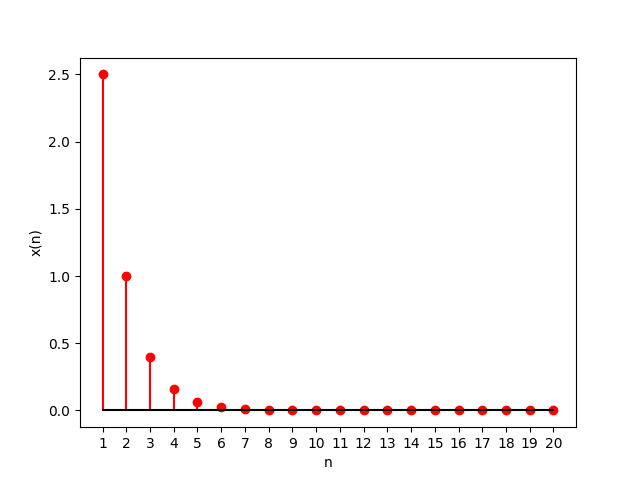
\includegraphics[width=\columnwidth]{ncert-maths/11/9/3/12/figs/graph1.png}
    \caption{stem plots of GP if $r=\frac{2}{5}$}
    \label{fig:11.9.3.12_1}
\end{figure}
\begin{figure}[h!]
    \centering
    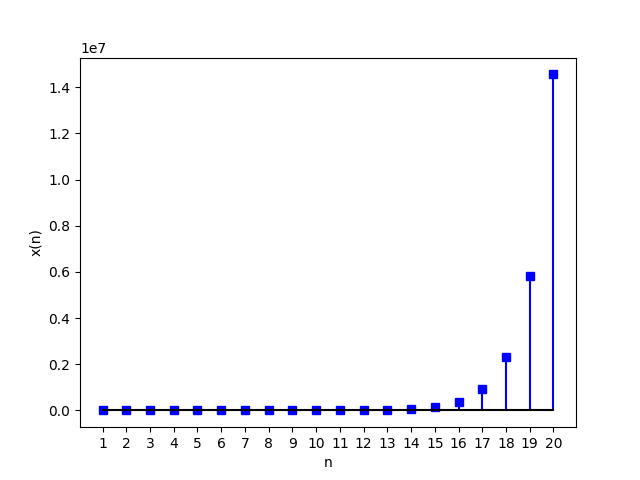
\includegraphics[width=\columnwidth]{ncert-maths/11/9/3/12/figs/graph2.png}
    \caption{stem plots of GP if $r=\frac{5}{2}$}
    \label{fig:11.9.3.12_2}
\end{figure}
%\end{document}

